%% paper.tex


%\documentclass[pldi]{sigplanconf-pldi16}
\documentclass[10pt]{sigplanconf}
% standard LaTeX packages

% standard LaTeX packages
%\usepackage{changebar}

\usepackage{balance}
\usepackage{alltt}
\usepackage{amsmath}
\usepackage{balance}
\usepackage{booktabs}
\usepackage{fixltx2e}
\usepackage{graphicx}
\usepackage{boxedminipage}
\usepackage{hyperref}
\usepackage{nicefrac}
\usepackage{subfig}
\usepackage{xcolor}
\usepackage{setspace}
\usepackage{xspace}
\usepackage{multirow}
\usepackage{colortbl}
\usepackage{amsfonts} 
\usepackage{blindtext}
\usepackage{chngpage}
\usepackage{listings}
\usepackage{mathtools}
\usepackage{amssymb}
\usepackage{pifont}
%\usepackage{pgfplotstable}

\usepackage[linesnumbered, vlined, ruled]{algorithm2e}
% font selection
%\usepackage{courier}
%\usepackage[scaled]{helvet}
\usepackage{mathptmx}
\usepackage{times}

% custom packages for this paper
%\usepackage{double-blind}
\usepackage{shared-affiliation}

\usepackage[numbers,sort&compress,square]{natbib}
%\newcommand{\wenfei}[1]{\textcolor{red}{$<<$Wenfei: #1$>>$}}

\lstset{
  basicstyle=\tiny,
  columns=fullflexible,
  numbersep=5pt,
  numberstyle=\scriptsize,
  showstringspaces=false,
  escapeinside={/*@}{@*/},
  belowcaptionskip=1\baselineskip,
  language=C,
  showstringspaces=true,
  keywordstyle=\bfseries,
  commentstyle=\itshape,
}


%\pgfplotstableset{
%    color cells/.style={
%        col sep=comma,
%        string type,
%        postproc cell content/.code={%
%                \pgfkeysalso{@cell content=\rule{0cm}{2.4ex}\cellcolor{black!##10}\pgfmathtruncatemacro\number{##1}\ifnum\number>5\color{white}\fi##1}%
%                },
%        columns/x/.style={
%            column name={},
%            postproc cell content/.code={}
%        }
%    }
%}


\makeatletter
\def\@copyrightspace{\relax}
\makeatother

\captionsetup{format=default, font=bf}


\newcommand*{\Scale}[2][4]{\scalebox{#1}{$#2$}}%
\newcommand{\comment}[1]{{}}

%% taken from unknown.sty
%\DeclareCaptionType{copyrightbox}

\sloppy

\input macros.tex

\begin{document}


\twocolumn[
\begin{@twocolumnfalse}
\begin{center}
{\Large\bf Learning from Big Malwares}
\end{center}
\smallskip
\centerline{
}
%\smallskip
\centerline{}

\smallskip
\end{@twocolumnfalse}
]



\begin{abstract}
\input section/abstract.tex
\end{abstract}


\section{Introduction}

As a free online service, VirusTotal~\cite{virustotal} analyzes files submitted by real-world users to identify many different kinds of malwares, 
like viruses, worms, trojans, and so on. 
VirusTotal applies different antivirus engines to each submitted file and generate an aggregated reports. 
All submitted files and generated reports are saved and can be accessed through public API. 

The repository on VirusTotal provides a good source to conduct data mining. 
Firstly, there are huge amount of data on VirusTotal.
Figure~\ref{fig:subnum} shows that there were more than 40 million suspicious files 
submitted last November. 
This amount of data makes VirusTotal a rough estimation of malwares in the real world. 
Secondly, all data on VirusTotal are labeled by state-of-the-art antivirus techniques. 
VirusTotal updates each antivirus engine every 5 minutes. 
Besides whether a given a submitted file is detected by an antivirus engine, VirusTotal also keeps exact detection tag returned by each engine. 
There are also online active malware researchers, 
who can comment and vote each submitted file and serve as an important supplement of antivirus engines. 
We believe mining data on VirusTotal could enable many ``Big Security'' applications. 

In industry, antivirus vendors widely use VirusTotal to identify false negatives and false positives of their products. 
They only utilize VirusTotal reports separately for each single suspicious file, but fail to leverage the whole repository. 
In academia, researchers began to pay attention to correlations among different VirusTotal reports. 
For example, {\bf [ToDo: discuss Heqing's work]}
We believe there are much more research opportunities through mining VirusTotal. 

In this paper, we view data on VirusTotal as a stream, based on each file’s submission time, and design two stream mining applications: 
\textit{hot malware family mining} and \textit{malware prediction}. 
There are possibly infinite malware families. 
Hot malware family mining can precisely identify malware families, 
which occupy more than a given percentage of total malwares, by using a constant number of counters.
Malwares does not appear uniformly across different malware families or across time, 
and they appear in bursts. 
We built a cache-based algorithm to predict malwares in which families would appear in the near future. 

\begin{figure}[t!]
\begin{center}
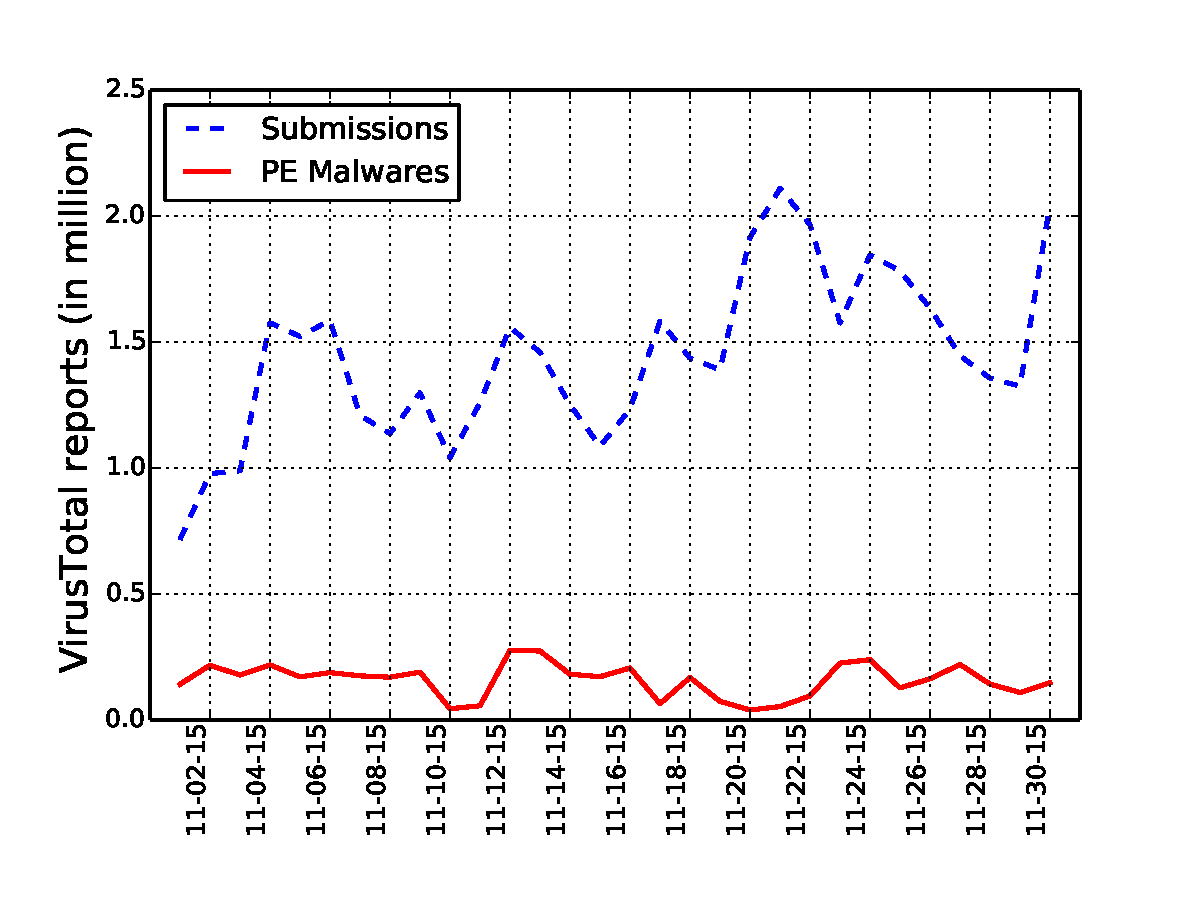
\includegraphics[width=3.0in]{figure/nov}
\caption{The number of files submitted to VirusTotal last November. }
\label{fig:subnum}
\end{center}
\end{figure}

In summary, we made the following contributions in this paper:

\begin{itemize}

\item We collect data submitted to VirusTotal last November, 
and briefly analyze these data to understand the characteristics of VirusTotal repository (Section~\ref{sec:meth}). 
\item We build two stream mining applications, one could identify hot malware family in a constant number of counters (Section~\ref{sec:hot}), 
and the other could predict malwares in the near future (Section~\ref{sec:predict}). 
Experimental results show that we can cover all hot malware family with a very few false positives, and we can predict future malwares with a high precision.
\item We discuss the future research opportunities through mining data on VirusTotal (Section~\ref{sec:oppo}), 
and demonstrate the feasibility by using our experience of building stream mining applications. 

\end{itemize}





\section{Data Collection and Basic Properties}
\label{sec:meth}

This section discusses how we collected and preprocessed data from VirusTotal.
We will present the analysis of these data in the next two sections.

\begin{table}[h!]
\centering
\footnotesize
{
%\begin{tabular}{@{\hspace{3pt}}l@{\hspace{3pt}}|@{\hspace{3pt}}c@{\hspace{3pt}}}
\begin{tabular}{l|l}
\hline
Metadata Fields & Explanation \\
\hline                            
%\cline{1-1}
{\bf name}      & file name of the submitted sample \\
{\bf timestamp} & timestamp for when the submission was made \\
{\bf source\_country} & the country from which the submission was made \\
{\bf source\_id} & user id of whom made the submission\\
{\bf tags} & providing more specific information for each {\bf type}\\
{\bf link} & where to download the submitted sample \\
{\bf size} & file size \\
{\bf type} & file type \\
{\bf first\_seen} & when the same sample was first submitted \\
{\bf last\_seen} & when the same sample was last submitted \\
{\bf hashes} & including sha1, sha256, vhash, md5, and ssdeep\\
{\bf total} & how many engines analyze the sample\\
{\bf positives} & how many engines identify the sample as malicious \\
{\bf positives\_delta} & changes in {\bf positives} fields \\
{\bf report} & detailed detection report from each AV engine \\
%\multicolumn{2}{|l|}
\hline

\end{tabular}
}
\mycaption{tab:fields}{VirusTotal Metadata.}
{ 
Fields for each submission retrieved from the VirusTotal private API and their relation explanation.
}
\end{table}




We downloaded the metadata and malware reports of all submitted files in November 2015 using the APIs VirusTotal provides,
resulting in a total of 43 million reports.
Table~\ref{tab:fields} shows the metadata fields and their meaning. 

{\color{red} (Work 4)
Figure~\ref{fig:type} shows file type distributions for all submissions. 
{\em Portable Executable (PE)}  files have the largest number of submissions. 
For around 11.5\% submissions, VirusTotal cannot figure out their file types. 
Malwares on Android have the third largest number of submissions.  
Other popular file types include web pages, compressed files, pdf, images, and so on. 
}

In this paper, we only focus on PE files 
and leave the analysis of other types of malicious files for future work. 
We filter all downloaded metadata by the type field. 
{\color{red} (Writing 5)
If the type field is either ``Win32EXE'' or ``Win32DLL'' tag, we consider the record as a PE file. 
Antivirus engines may disagree with each other, so
we only rely on Microsoft antivirus engine to judge whether a PE file is a malware, because
Microsoft has a very good reputation in detecting PE malwares. 
}
Within the 43 million reports, 4.7 million are PE malwares. 
The number of reports, PE reports, and PE malwares submitted each day are shown in Figure~\ref{fig:subnum}.

{\color{red} (Writing 4)
Malwares can be classified into related clusters, according to their dynamic behaviors and static features. 
These clusters are referred to as malware families in our paper. }
The Microsoft antivirus engine classifies malwares into different names~\cite{microsoft}. 
We utilize this naming mechanism to decide what family a malware belong to.
Specifically, if two malwares have the same name under Microsoft engine, we consider them to be from the same family.

One caveat of VirusTotal is that it is possible that the VirusTotal APIs return redundant reports 
for the same submitted file. 
We use the combination of sha256 hash value and timestamp to detect and remove redundant reports.

After removing redundant reports, we find that most malwares were submitted only once to VirusTotal in November 2015. 
Out of the total 4.7 million PE malware submissions, 4 million are distinct. 
On average, each PE malware was submitted 1.17 times to VirusTotal in November 2015. 
This observation is in contradictory to the common belief that most malwares are encountered by more than one user.
We suspect that the reason behind this low degree of repeated submissions by different users in one month
is that VirusTotal users
tend to check whether their suspicious files have already been submitted recently
and avoid submitting redundant files.

{\color{red} (Work 3 and Work 5)
Figure~\ref{fig:size} shows the file size distribution for VirusTotal malwares. 
The smallest malware is only 704 bytes, and the largest one is more than 502\,MB. 
95.3\% of malwares fall into the range from 16\,KB to 2\,MB. 
VirusTotal does not provide tags to differ 64-bit malwares from 32-bit malwares directly. 
We sample 10000 malwares and download their executable binaries from VirusTotal.
We apply Linux command file to each sampled malware binary. 
64-bit malwares are labeled with PE32+ by file command. 
In total, there are only 127 64-bit malwares in our sample set, and all other malwares are 32-bit.
}

Similar to all previous empirical studies, all our findings, experimental results, 
and conclusions need to be considered with our methodology in mind. 

{\color{red} (Writing 6)
We only use one month of data as our first step in studying VirusTotal. 
We leave investigating longer period of time for future work. 
}
The VirusTotal APIs only track which submission reports are sent to each downloader approximately, 
and there is no guarantee that all submission reports on VirusTotal can be downloaded successfully. 
Thus, it is possible that we missed some malwares submitted to VirusTotal. 
Also, we only leverage Microsoft antivirus engines to decide whether or not a submission is malicious, 
and it is possible that Microsoft antivirus engines cannot make this decision precisely. 
How to get a precise label for a PE file is out of the scope of this paper.  
Although there is a huge amount of malwares on VirusTotal, we believe that there are malwares never submitted to VirusTotal, 
and there are malwares submitted much later than when they appear in the real world.
Since there are no conceivable ways to study these malwares,
we believe that the malwares in our study provide a representative malware sample of the real world. 




\section{Malware Metadata Study}
\label{sec:meta}

This section presents our study of VirusTotal malwares’ metadata. 
This part of our study is performed in 4 dimensions:

{\bf What?} What is file size distributions of malwares on VirusTotal? 
How many malwares are 32-bit, and how many malwares are 64-bit? 

\begin{figure}[t!]
\begin{center}
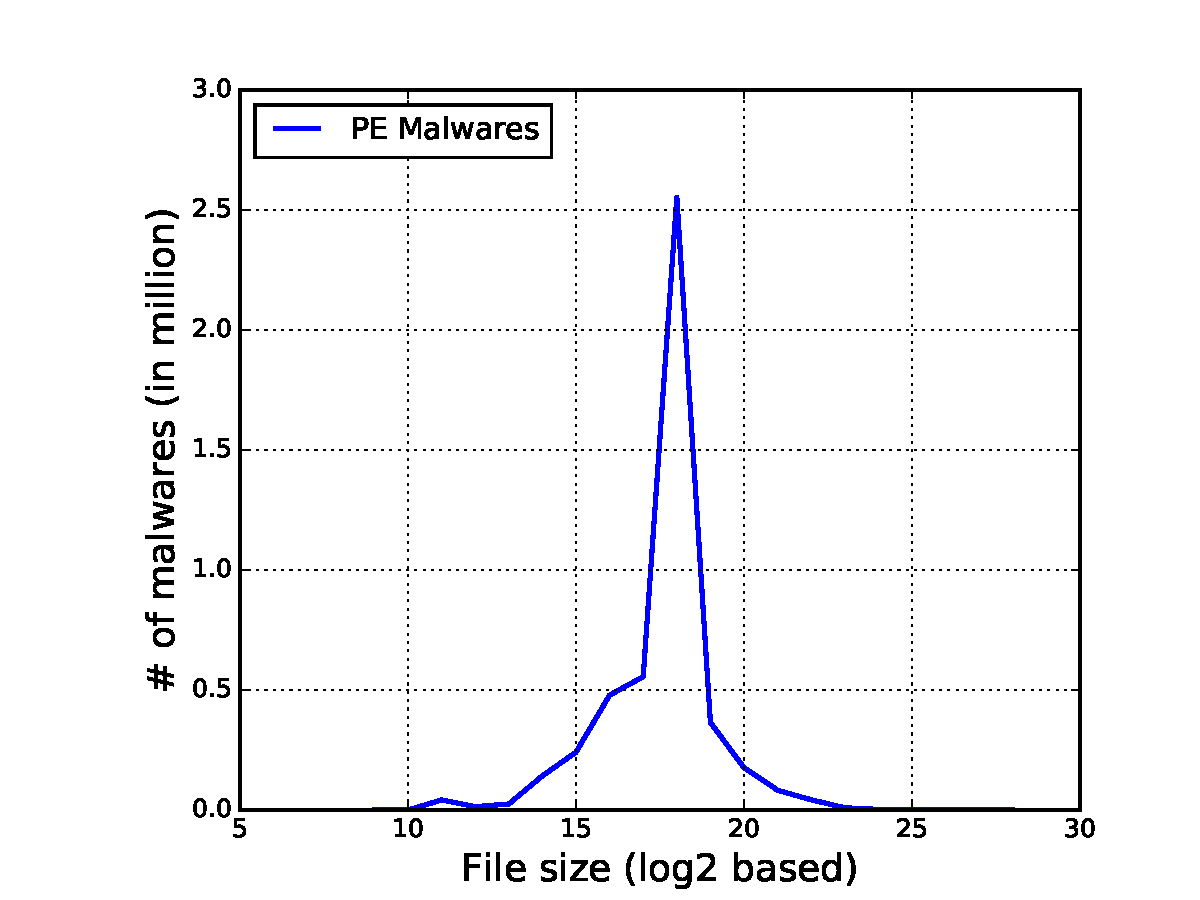
\includegraphics[width=2.5in]{figure/size}
\mycaption{fig:size}{Size distribution for malwares on VirusTotal in November 2015.}
{The number of malwares falling into each log2-based size category in November 2015.}
%\label{fig:new}
\end{center}
%\vspace{-0.3in}
\end{figure}

Figure~\ref{fig:size} shows the size distribution for malwares. 
The smallest malware is only 704 bytes, and the largest one is more than 502 MB. 
95.3\% of malwares fall into the range from 16 KB to 2 MB. 

VirusTotal does not provide tags to differ 64-bit malwares from 32-bit malwares directly. 
We sample 10000 malwares and download their executable binaries from VirusTotal.
We apply Linux command file to each sampled malware binary. 
64-bit malwares are labeled with PE32+ by file command. 
In total, there are only 127 64-bit malwares in our sampled set. 

{\bf Who?} How many real-world users submit malwares on VirusTotal? 
How malware submissions distribute among different users? 

\begin{figure}[t!]
\begin{center}
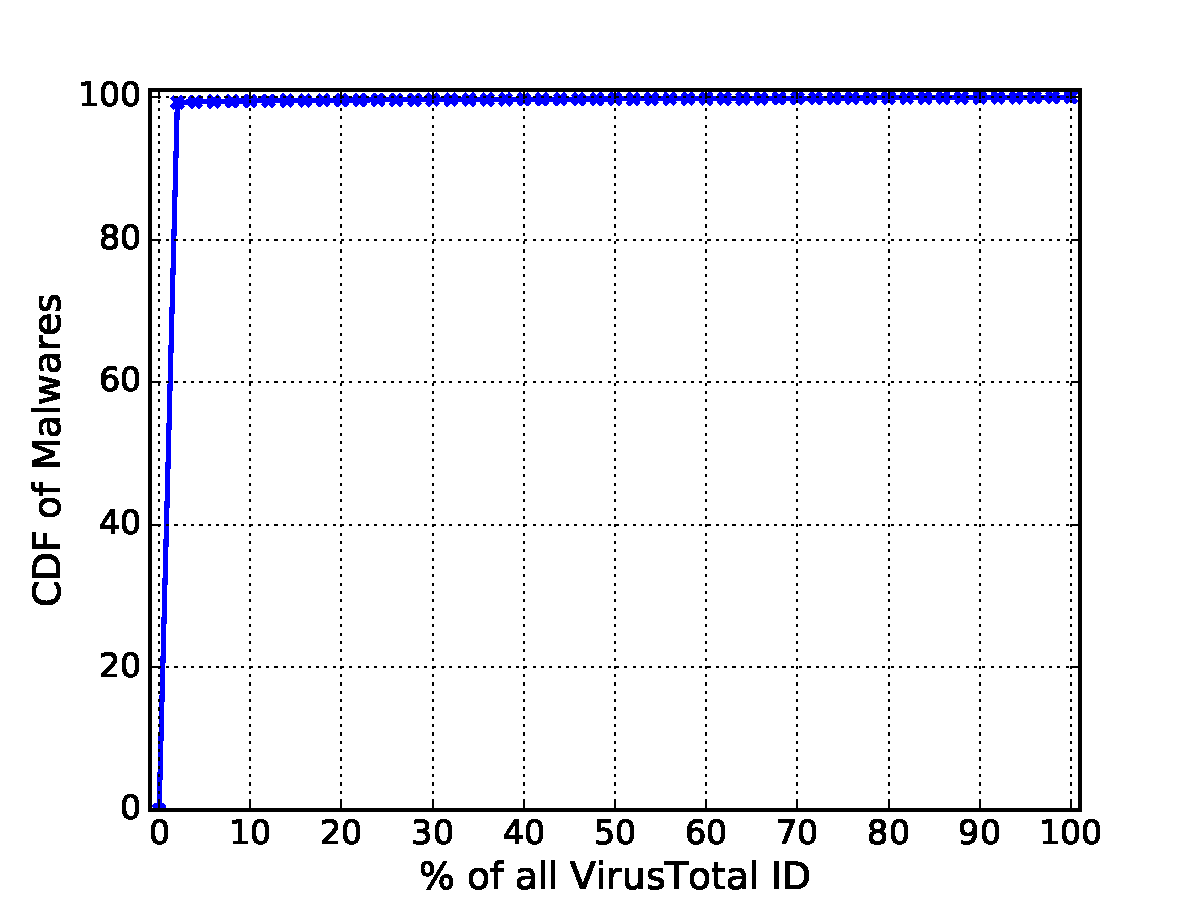
\includegraphics[width=2.5in]{figure/id}
\mycaption{fig:id}{Skewness of malware submissions from different users in November 2015.}
{Accumulation distribution of malwares submitted by different users in November 2015.}
%\label{fig:acum}
\end{center}
\vspace{-0.25in}
\end{figure}

For around 0.6 million malwares, VirusTotal fails to provide their submission IDs. 
The left 4 million malwares are submitted by 20739 distinct users.
As shown in Figure~\ref{fig:id}, malware submissions are distributed unbalanced among different users.
15748 users only submit one malware. 
The user, with largest submission number, submitted more than 3 million malwares. 

{\bf Where?} Where do malware submissions come from? 

\begin{figure}[t!]
\begin{center}
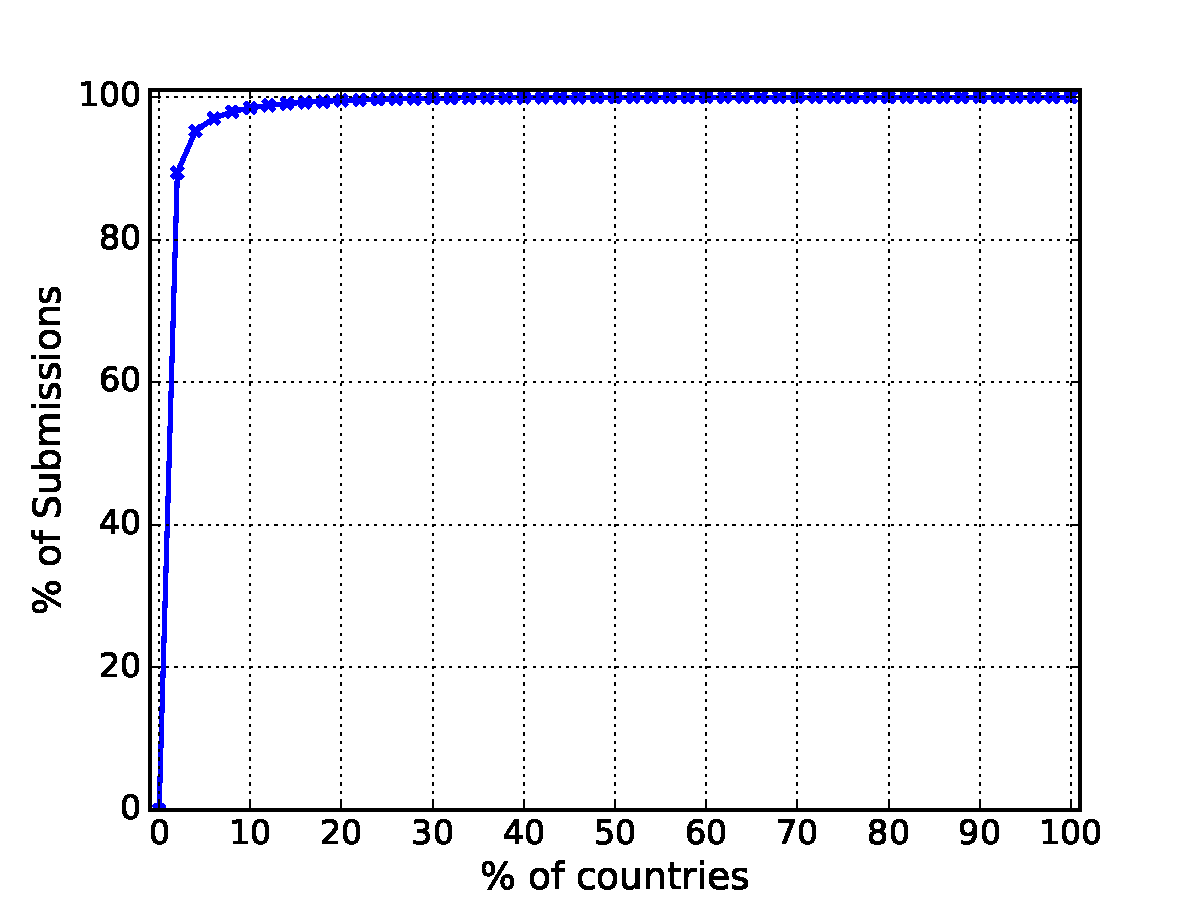
\includegraphics[width=2.5in]{figure/country}
\mycaption{fig:country}{Skewness of malware submissions from different countries in November 2015.}
{Accumulation distribution of malwares submitted from different countries in November 2015.}
%\label{fig:acum}
\end{center}
\vspace{-0.25in}
\end{figure}

There are also around 0.6 million malwares, 
whose submission countries VirusTotal fails to provide. 
All other malwares are submitted from 164 distinct countries. 
The top 5 countries are Canada, USA, China, France, and Germany. 
As shown in Figure~\ref{fig:country}, 
malware submissions are also distributed unbalanced among different countries. 

{\bf When?} How life-time distributes for malwares submitted to VirusTotal? 
Specifically, how long is it between submission time and when malwares firstly seen on VirusTotal?

\begin{figure}[t!]
\begin{center}
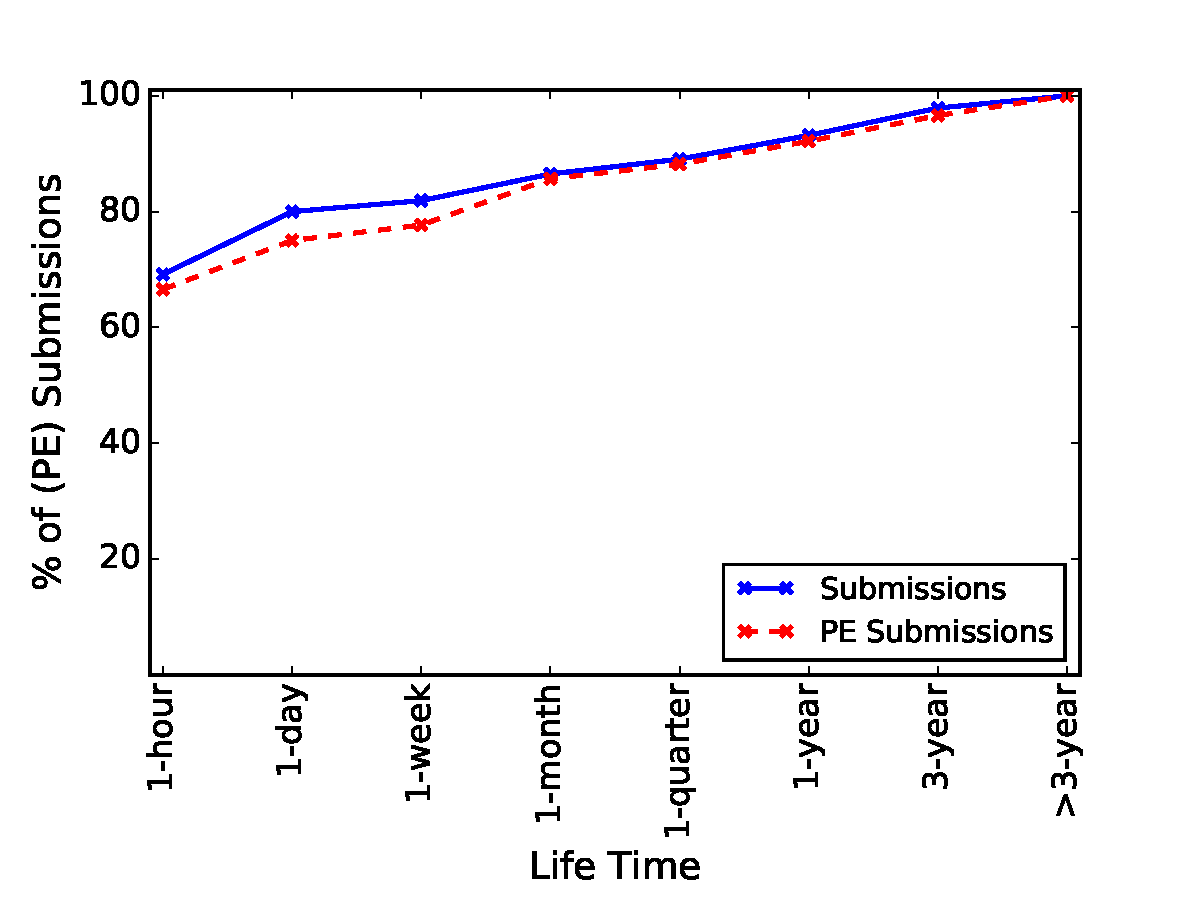
\includegraphics[width=2.5in]{figure/lifetime}
\mycaption{fig:life}{Malwares' lifetime in November 2015.}
{Accumulation distribution of malwares' lifetime in November 2015.}
%\label{fig:acum}
\end{center}
\vspace{-0.25in}
\end{figure}

As shown in Figure~\ref{fig:life}, malwares submitted to VirusTotal are quite new. 
More than 75\% malware submissions are firstly seen on VirusTotal.
For more than 90\% malware submissions, 
their submission time is less than one month since it was firstly seen on VirusTotal.  
\section{Malware Temporal Properties}
\label{sec:temporal}

This section presents our study of the temporal properties of VirusTotal malwares
and answers three fundamental questions: 
how many malware families appear everyday, 
{\color{red} (Work 2)
what lifetime of malwares on VirusTotal distributes,  
}
and whether or not malwares occur in bursts.
To answer the last question, we design a new caching mechanism 
that can be used for both offline and online malware predictions.
This cache-based malware prediction technique can predict which malware families will appear in the near future with high precision.

\begin{figure*}[!htb]
\minipage{0.31\textwidth}
  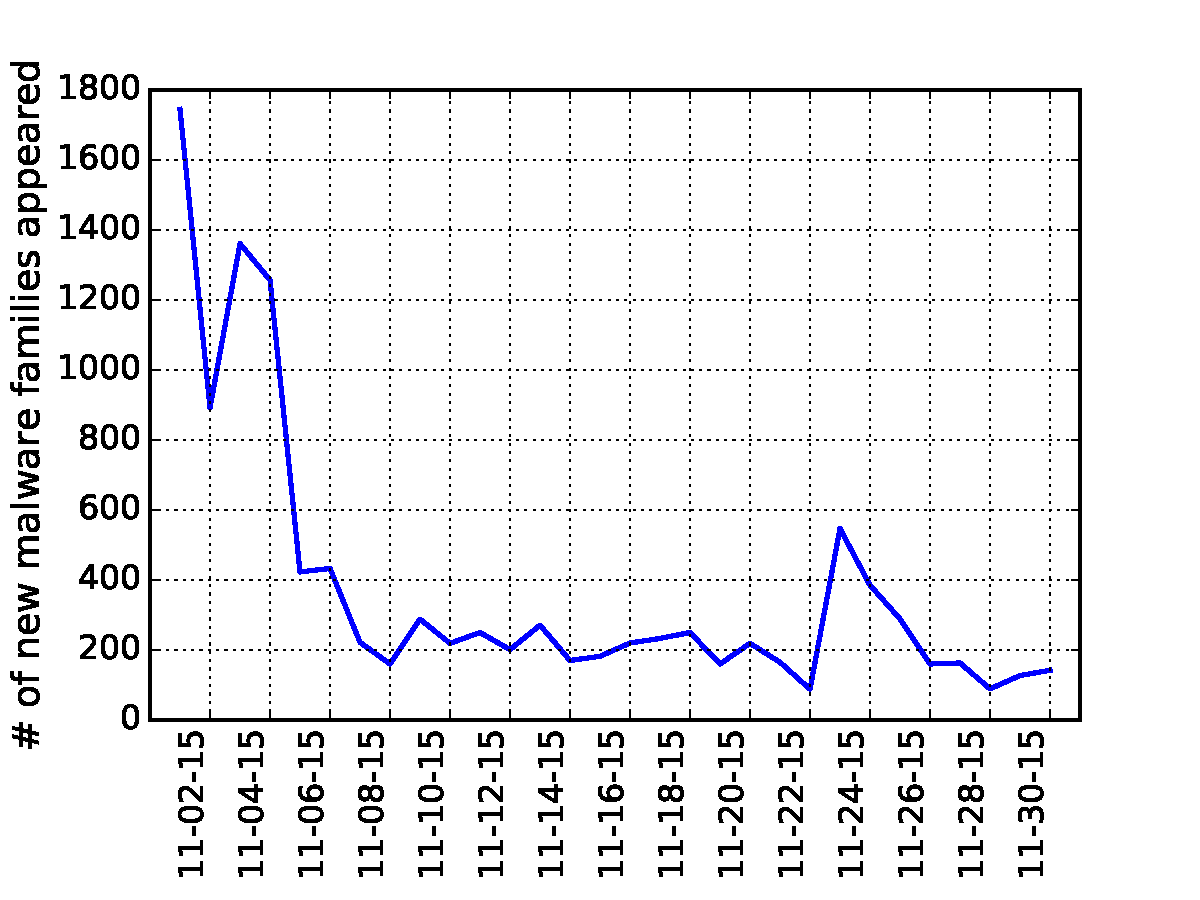
\includegraphics[width=\linewidth]{figure/new_family}
\mycaption{fig:new}{New malware families on VirusTotal in November 2015.}
{
The number of new malware families we observed every day in November 2015.
}
  %\label{fig:overlap}
\endminipage\hfill
\minipage{0.31\textwidth}
  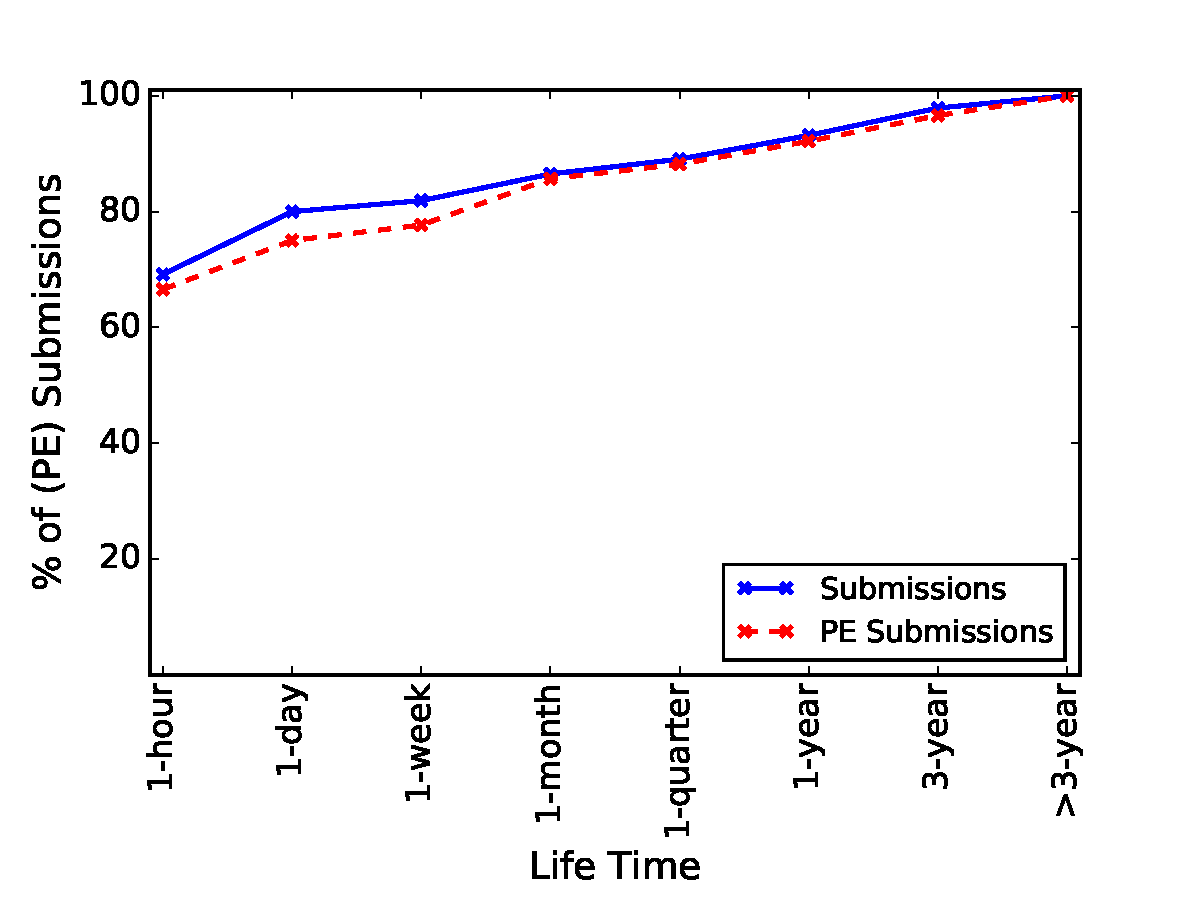
\includegraphics[width=\linewidth]{figure/lifetime}
 \mycaption{fig:life}{Malwares' lifetime in November 2015.}
{
Cumulative distribution of lifetime for malwares with more than one submission in November 2015.
}
  %\label{fig:maxUncover}
\endminipage\hfill
\minipage{0.31\textwidth}%
  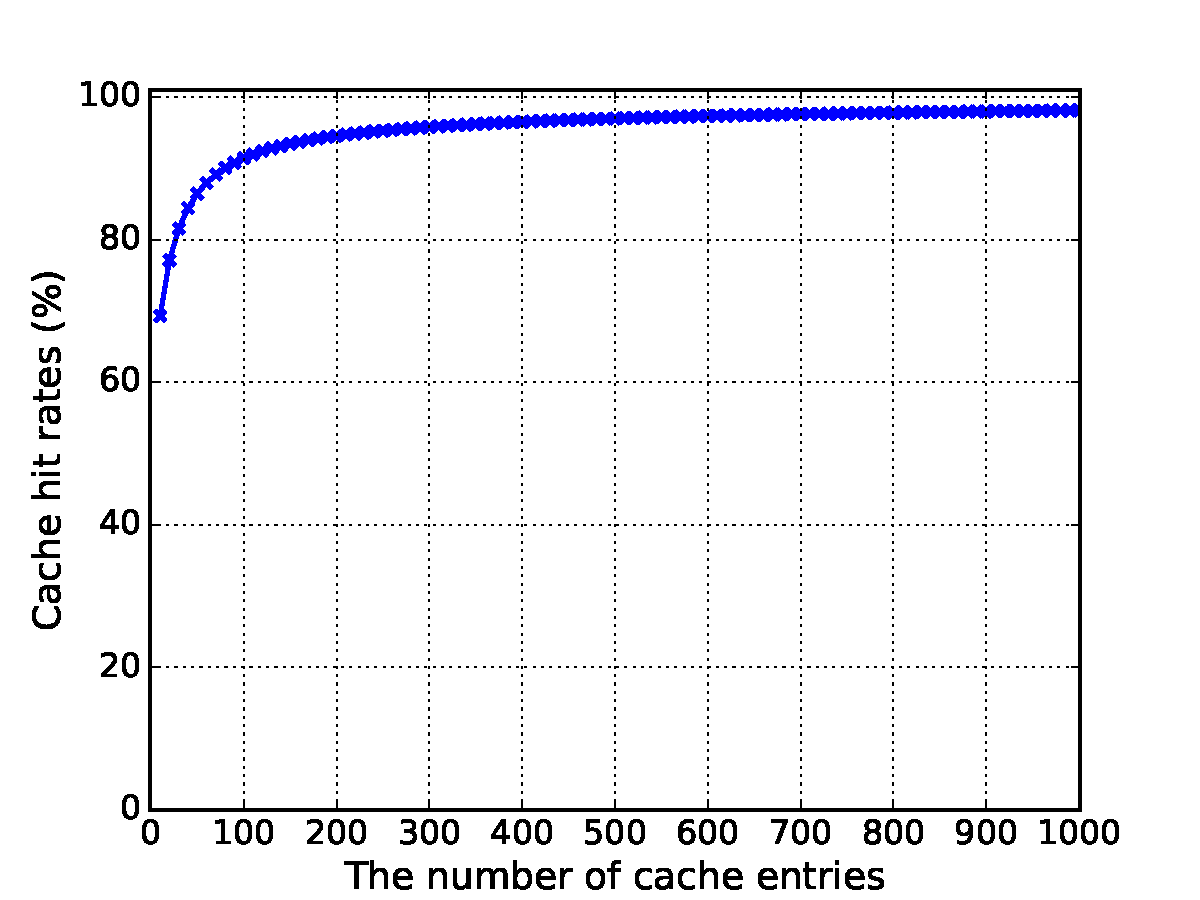
\includegraphics[width=\linewidth]{figure/LRU}
  \mycaption{fig:cache}{Relation between cache hit rate and cache size.}
{Cache hit rate under different values of cache size from 10 to 1000.}
  %\label{fig:aveUncover}
\endminipage\hfill

\vspace{-0.1in}
\end{figure*}

\begin{figure*}[!htb]
\minipage{0.31\textwidth}
  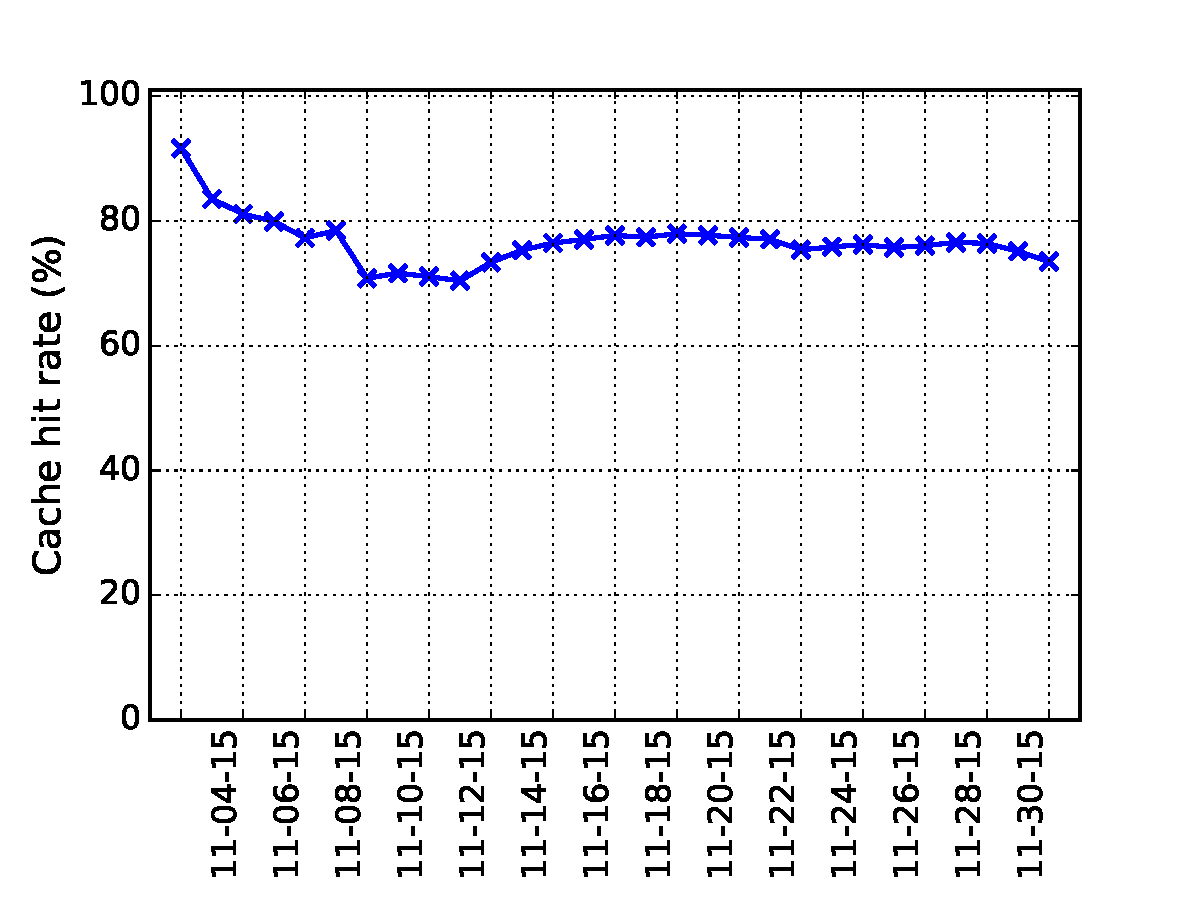
\includegraphics[width=\linewidth]{figure/LRU_day}
\mycaption{fig:batchcache}{Cache hit rate in November 2015.}
{
Cache hit rate every day in November 2015 if we only update cache content at the end of every day.
}
  %\label{fig:overlap}
\endminipage\hfill
\minipage{0.31\textwidth}
  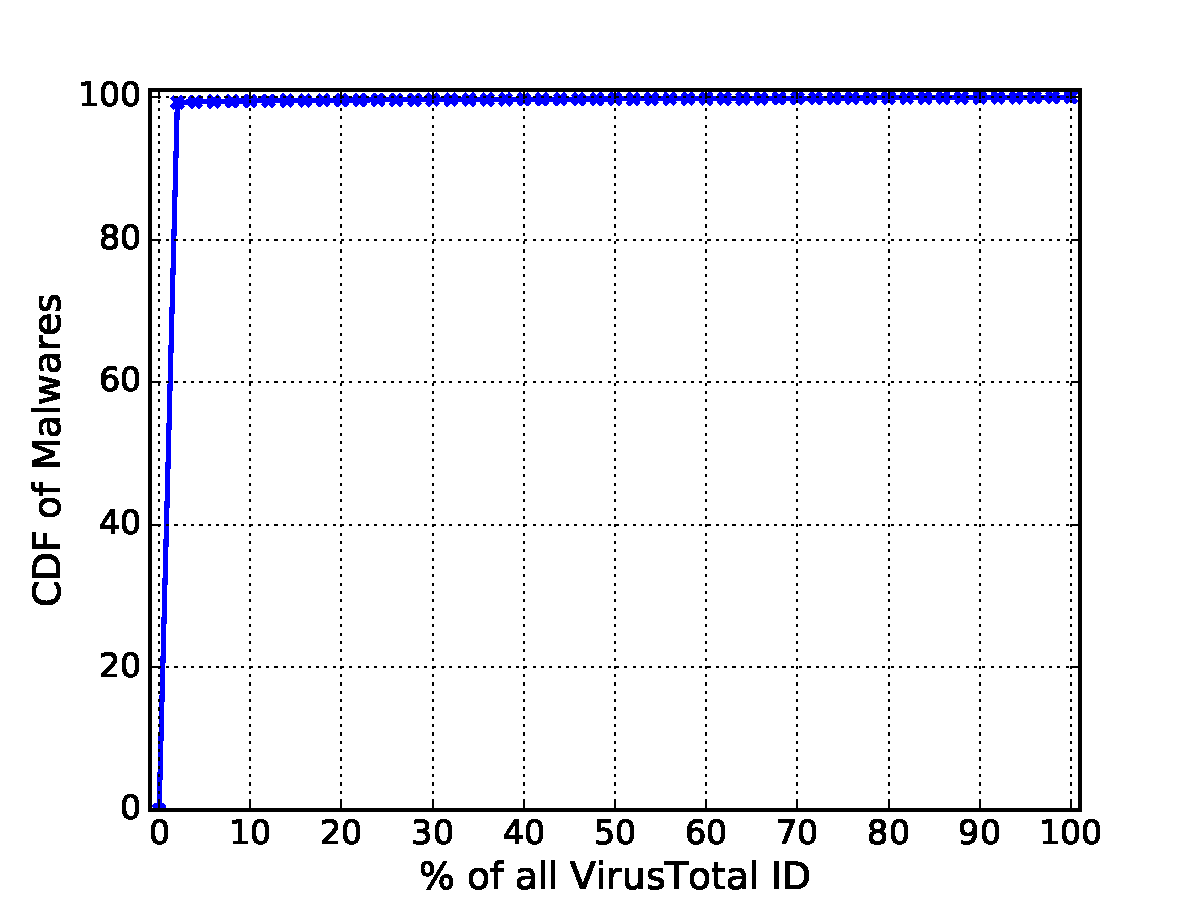
\includegraphics[width=\linewidth]{figure/id}
 \mycaption{fig:id}{Skewness of malware submissions from different users in November 2015.}
{Cumulative distribution of malwares submitted by different users in November 2015.}
  %\label{fig:maxUncover}
\endminipage\hfill
\minipage{0.31\textwidth}%
  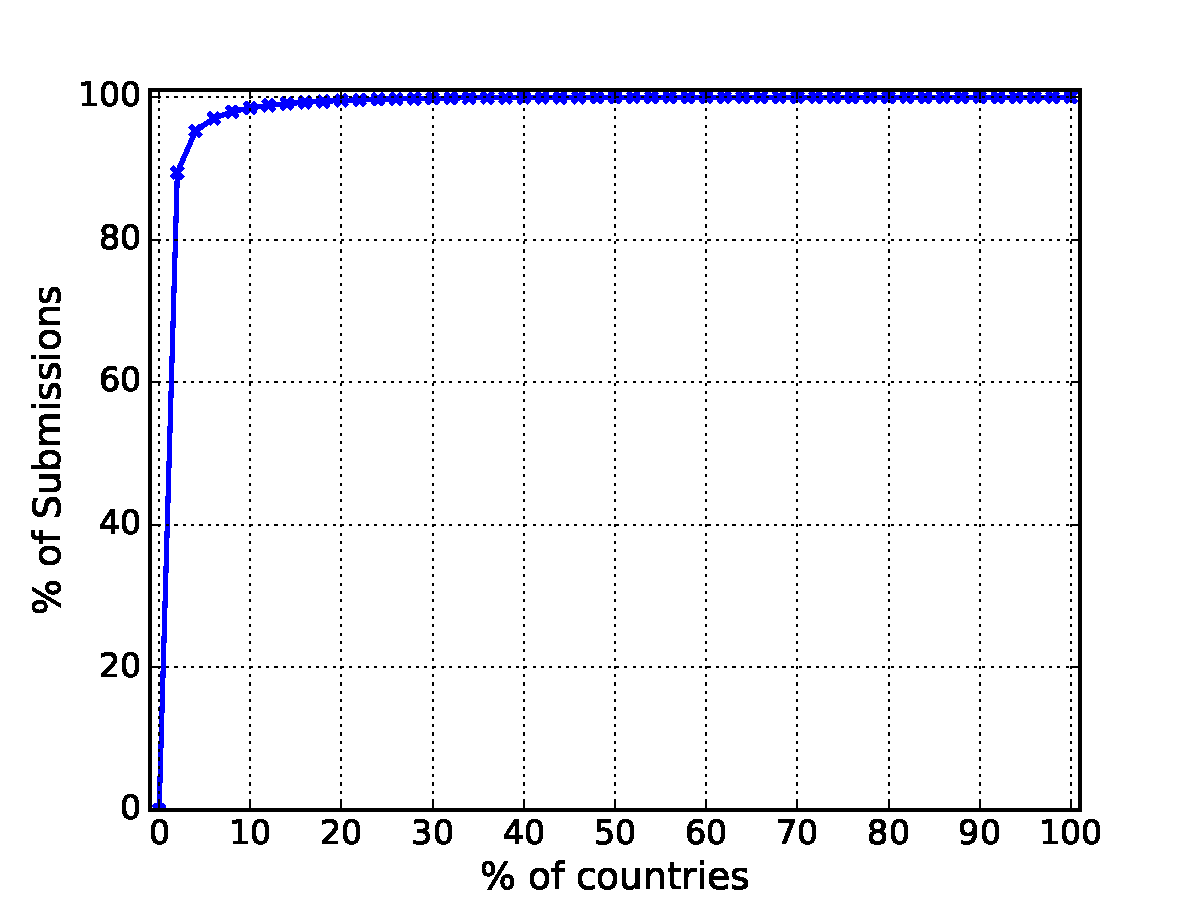
\includegraphics[width=\linewidth]{figure/country}
  \mycaption{fig:country}{Skewness of malware submissions from different countries in November 2015.}
{Cumulative distribution of malwares submitted from different countries in November 2015.}
  %\label{fig:aveUncover}
\endminipage\hfill

\vspace{-0.1in}
\end{figure*}

We first study how many new malware families appear everyday. 
Figure~\ref{fig:new} shows the number of new malware families appearing on each day in November 2015. 
Since we do not include data before November 1, 
there are more new malware families in the first few days.
After that, the number of new malware families becomes stable, 
falling into a range between 100 and 400. 
In total, there are 11302 malware families in this time period. 

{\bf Observation 1:} 
{\em 100-400 new malware families appear each day.}

%\begin{figure}[t!]
\begin{center}
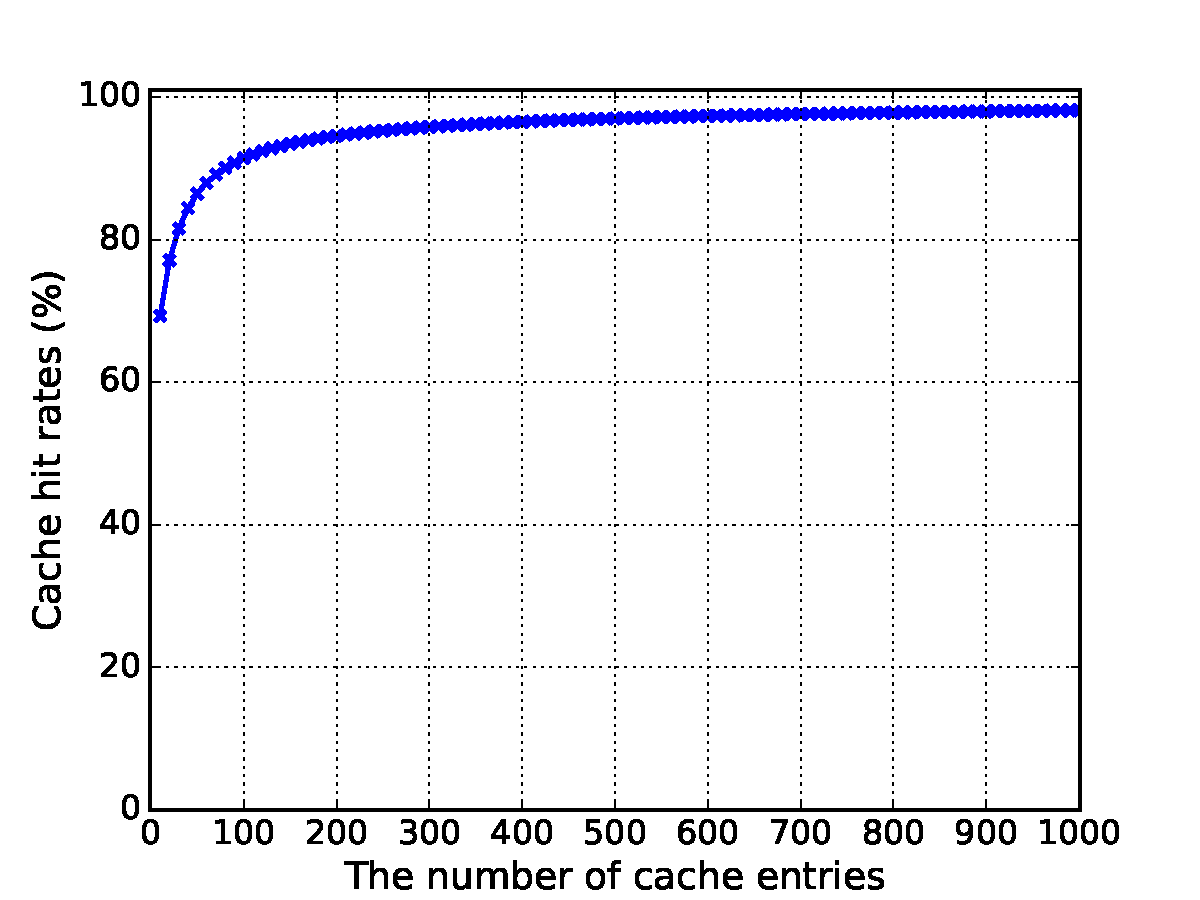
\includegraphics[width=2.5in]{figure/LRU}
\mycaption{fig:cache}{Relation between cache hit rate and cache size.}
{How cache hit rate changes with the change of cache size from 10 to 1000.}
%\label{fig:cache}
\end{center}
\end{figure}
%\begin{figure}[t!]
\begin{center}
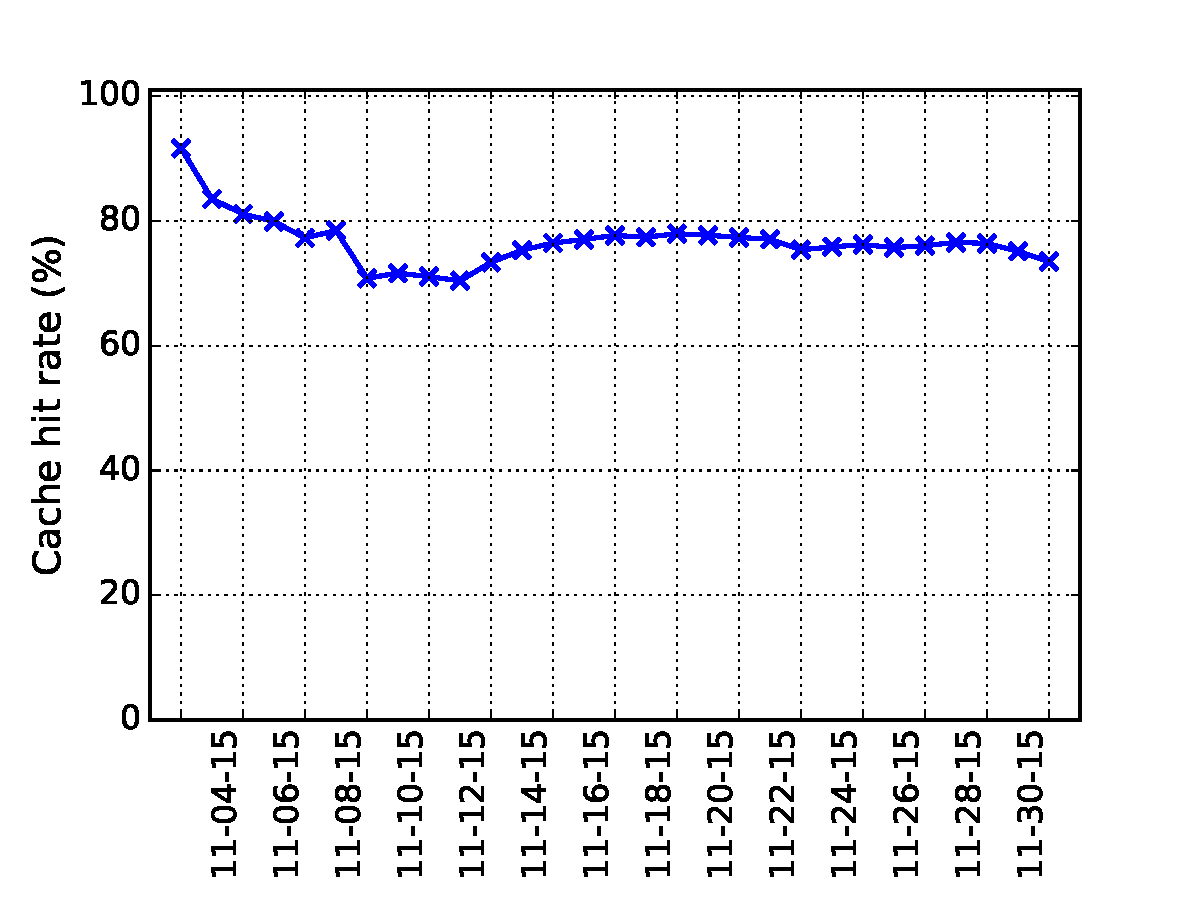
\includegraphics[width=2.5in]{figure/LRU_day}
\mycaption{fig:batchcache}{Cache hit rate in November 2015.}
{Cache hit rate every day in November 2015 if we only update cache content at the end of every day.}
%\label{fig:batchcache}
\end{center}
\vspace{-0.1in}
\end{figure}



{\color{red} (Work 2)
An interesting property worth studying is how long a malware lives. 
Finding the exact answer to this question is extremely difficult, since there 
is no log of when a malware comes into existence and when it extincts.
Here, we use the VirusTotal data to have a peek into this question.
Specifically, we use the tiem span from when the first submission of a malware to VirusTotal happens
to the time of its last submission
to provide a rough estimation of the life time of this malwares.
Figure~\ref{fig:life} plots the cummulative distribution of the calculated submission time span of malwares with more than one submission.
89.68\% malwares are only submitted once.
Other than these malwares, 0.004\% malwares have submission span within an hour, 
0.17\% span from one hour to one day, and 8.39\% span more than one week.


{\bf Observation 2:}
{\em A fair amount of malwares live longer than one week.} % need to conclude this based on the above numbers

}


Finally, we investigate whether malwares behave temporal locality.
Temporal locality is an important metric that can guide the 
prediction of near-future malwares.

Specifically, we analyze how bursty malwares in the same family appear.  
Inspired by previous usage of cache mechanisms in predicting bugs~\cite{predicting},
we design a new cache mechanism to study the burstiness of malwares.

This caching mechanism can be used to analyze historical malware reports offline 
as well as to analyze online malwares and predict near-future malware occurrences.

We view malware submission reports as a stream of inputs 
and feed the stream into a cache. 
Each input (\ie, each report) is associated with an address (the family it belongs to) and a time (the submission time of the file).
Thus, a cache hit means that the new report belongs to a family that is currently in the cache,
\ie, the new input has the same address as an entry in the cache.
Therefore, a high cache hit rate implies that the occurrence of malwares exhibit temporal locality.

As with general cache mechanisms such as CPU caches and file system buffer caches, 
there are several parameters to tune in a cache.
The cache block size, or cache line size, controls the granularity of cache management, 
\ie, how many entries are inserted into and evicted from cache together.
Cache prefetching loads spatially close entries into caches in advance. 
Cache replacement policy controls what entries to evict when cache is full.
{\color{red} (Writing 9)
We use a simple cache setting in our evaluation. 
We fix the cache block size to be one, no prefetching, 
and use the LRU replacement policy.
We leave the exploration of the effect of other cache configurations for future work. 

Our malware family cache works as follows.
We start with an empty cache. 
For a new file submission, if the malware family is already in the cache, 
we move the hit cache entry to the front of our cache entry list. 
If the new malware family is not in the cache, 
we create a new cache entry and add it to the front of the cache entry list.
If the cache is full, we evict the entry at the end of the list. 
%The cache hit rate is calculated as follows: 
}

%$$ \mbox{hit rate} = \dfrac{\mbox{\# of hits}}{\mbox{\# of hits + \# of misses}}$$

We implemented this malware family cache using Python
and conducted experiments on an AWS c4.4xlarge virtual machine, 
which contains 16 virtual CPUs and 30\,GB memory.

We conducted two experiments. 
The first experiment explores how the cache hit rate changes with the number of cache entries. 
We change the cache size from 10 to 1000. 
As shown in Figure~\ref{fig:cache}, the hit rate grows from 69.31\% to 98.14\%. 
When using more than 80 cache entries, which is less than 1\% of the total number of malware families, the cache hit rate rises above 90\%, 
and when using more than 230 cache entries, which is less than 3\% of the total number of malware families, 
the cache hit rate rises above 95\%. 
{\color{red} (Writing 8)
The high cache hit rate and the small cache size confirm that malwares occur in bursts.
}

{\bf Observation 3:} 
{\em The occurrence of malwares in each family has strong temporal locality.}  

{\color{red} (Writing 7)
In offline prediction, malwares encountered in each client site are merged together. 
These data are used to predict which malware family would appear in the near future in a large scale.
Malwares encountered in one client site can be viewed as a random sample of all malwares. 
If we can predict malware occurrence online, we could apply personalized defense mechanism and malware detection mechanism on the client side. 
}
To support online malware occurrence prediction, it is essential to lower the 
performance overhead of running our cache mechanism.
To this end, we lower the cache content update frequency from once per malware report to once per day.
That is, we keep cache content unchanged to count cache hits and cache misses each day and update the cache content at the end of each day.
In this second experiment, we fix the cache size to 200. 
{\color{red} (Writing 1)
Figure~\ref{fig:batchcache} shows prediction rate by using next day’s data. 
Most cache hit rate is above 70\%,
showing that even when lowering performance overhead, \ie, updating cache content once a day, 
our cache mechanism still achieves a good estimation of malware occurrences.
}   
{\color{red} (Writing 9)
We do not need to combine malwares encountered in each client site and send out updated cache content frequently. Cache-based malware prediction can be used in an online scenario. 
}

{\color{red} (Work 6)
We also study which malware families cause more cache misses 
and have bad prediction results. 
We count cache misses for each malware family, 
and consider a family with more than half malwares causing cache misses as family with bad prediction results. 
We find that whether a family has bad prediction results is related to the number of malwares it contains. 
When cache size is 100, the largest number of malwares contained in one family with bad prediction results is 2307. 
When cache size is 1000, the largest number of malwares contained in one family with bad prediction results is 126. 
}



\section{Malware Distribution}
\label{sec:dist}

%\begin{figure}[t!]
%\begin{center}
%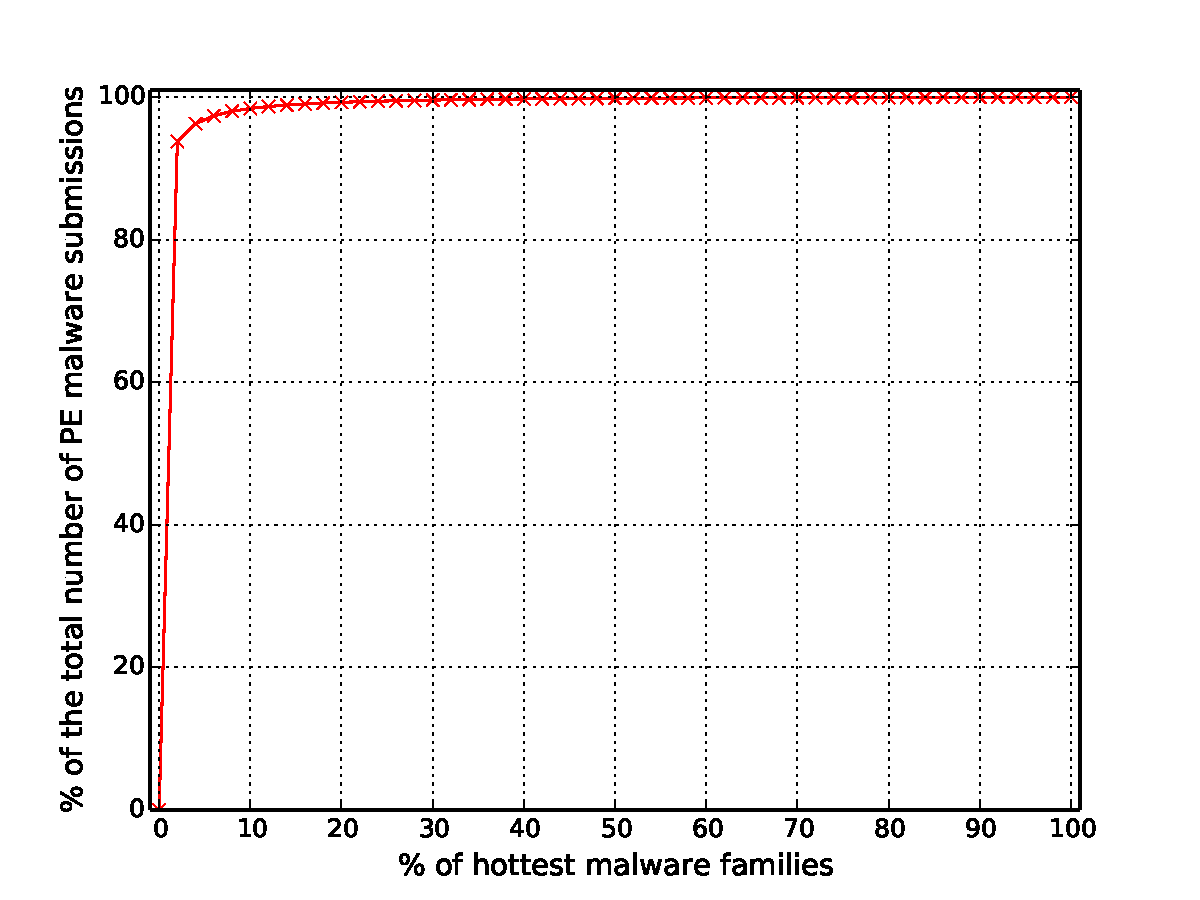
\includegraphics[width=2.5in]{figure/cum}
%\caption{Skewness of malware families appearing in November 2015.}
%\label{fig:acum}
%\end{center}
%\end{figure}






\begin{figure*}[!htb]

\minipage{0.31\textwidth}%
  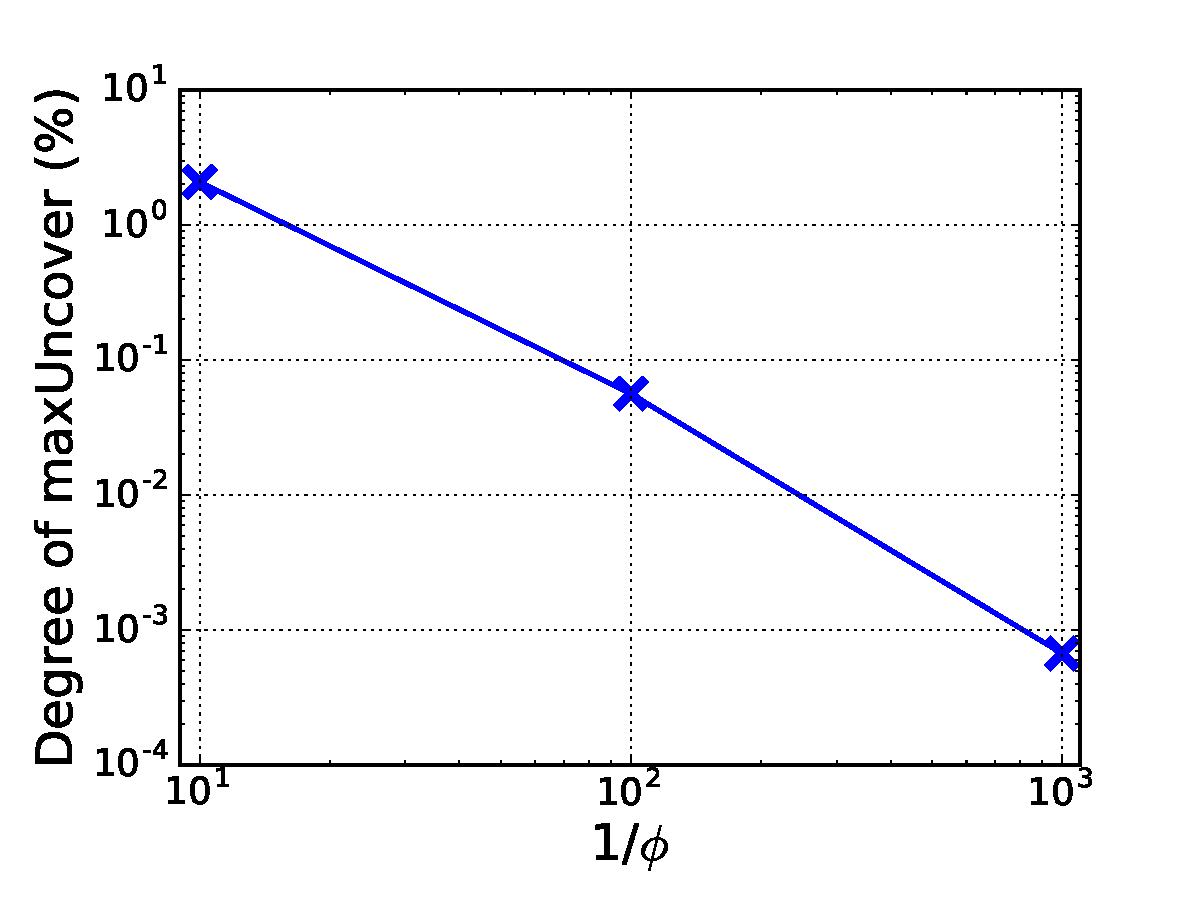
\includegraphics[width=\linewidth]{figure/maxUncover.pdf}
  \mycaption{fig:maxUncover}{Relation between $\phi$ and degree of maxUncover.}
  {
  How the degree of maxUncover changes with the change of $\phi$ from $10^{-1}$ to $10^{-3}$.
  }
  %\label{fig:aveUncover}
\endminipage\hfill
\minipage{0.31\textwidth}%
  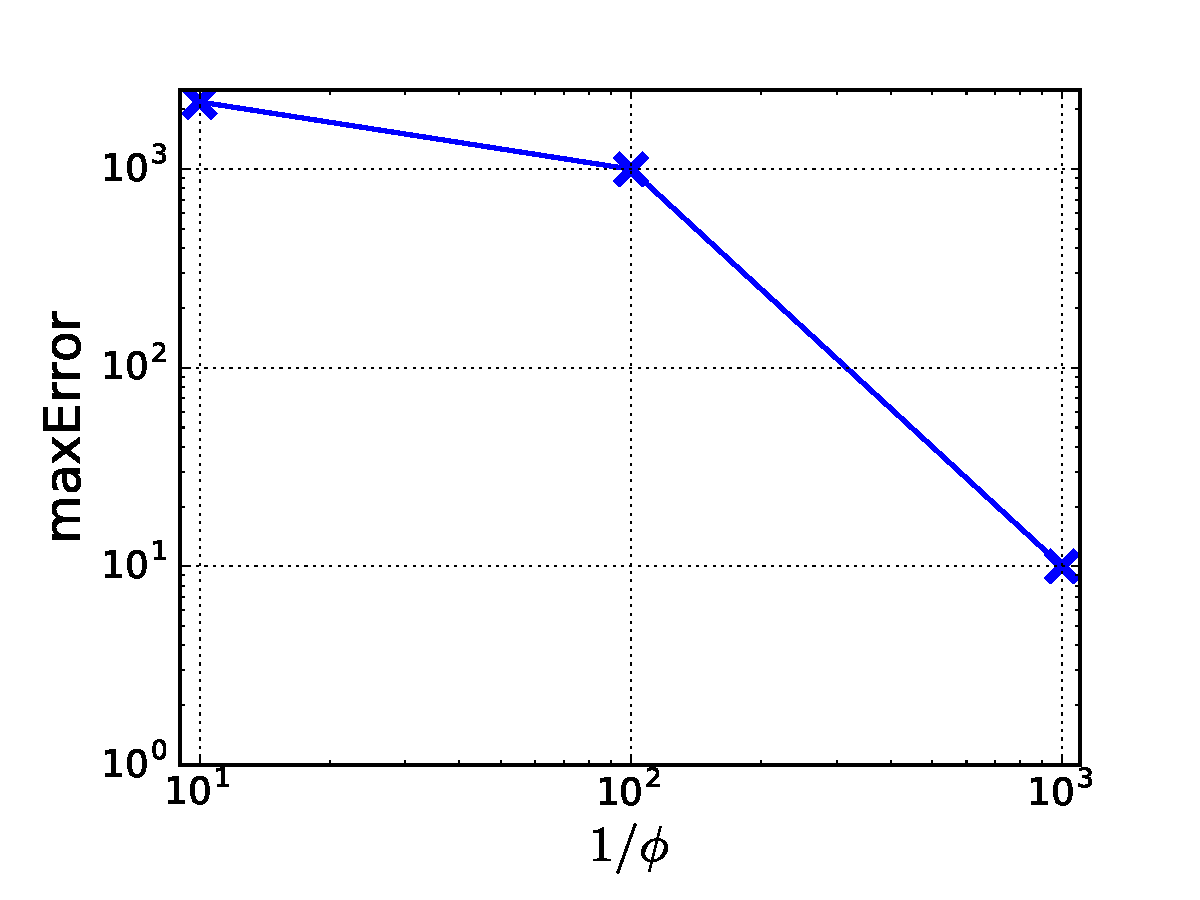
\includegraphics[width=\linewidth]{figure/maxError.pdf}
  \mycaption{fig:maxError}{Relation between $\phi$ and maxError.}
  {How maxError changes with the change of $\phi$ from $10^{-1}$ to $10^{-3}$.}
  %\caption{Relation between $\phi$ and maxError.}
  %\label{fig:maxError}

\endminipage\hfill
\minipage{0.31\textwidth}%
  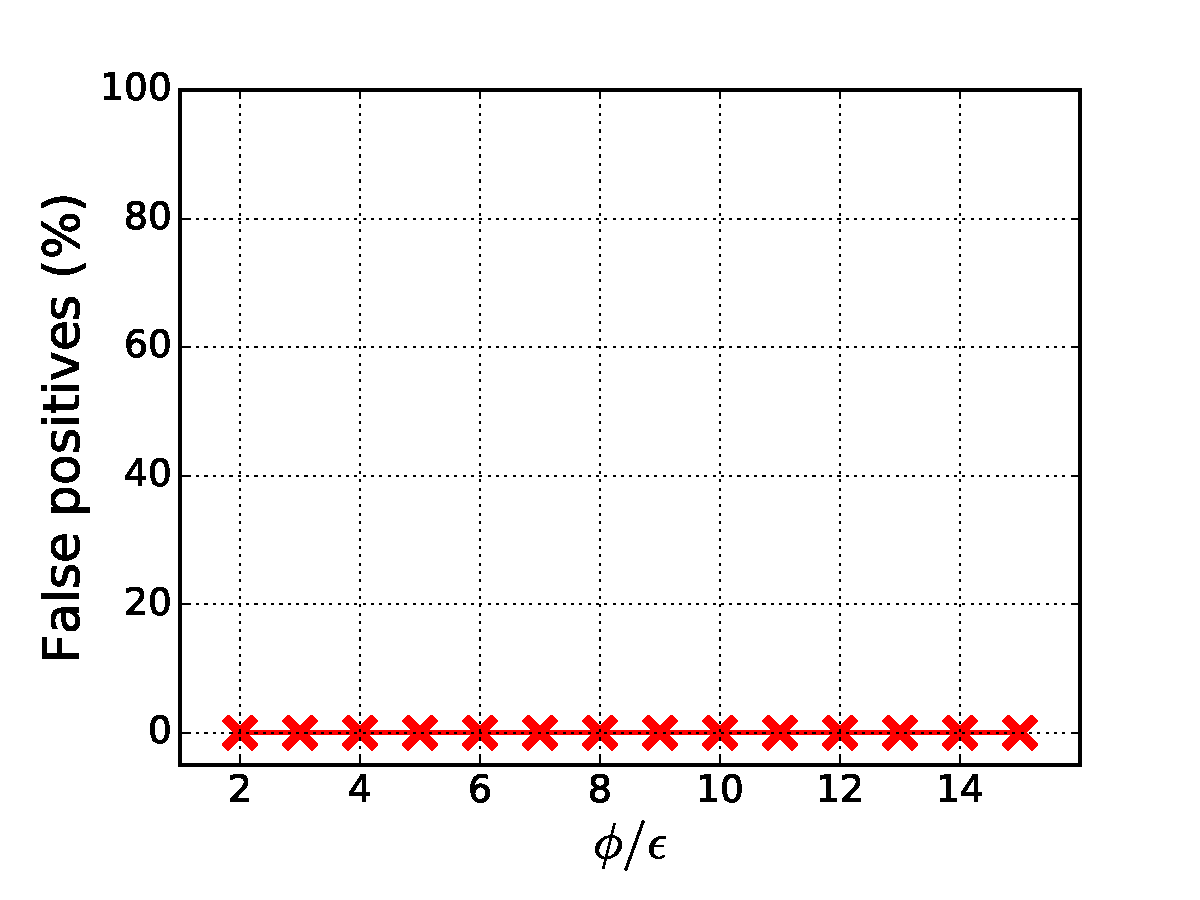
\includegraphics[width=\linewidth]{figure/fp}
  \mycaption{fig:fp}{False positives.}
{False positives in $(\phi, \epsilon)\mbox{-}HMF$ as a function of $\epsilon$. The value of $\phi$ is fixed to $10^{-2}$.
The value of $\phi/\epsilon$ changes from 2 to 15.}
  
\endminipage
\vspace{-0.1in}
\end{figure*}


%{\color{red} (Work 1)
This section presents our study on how malwares distribute in countries and malware families.

%4 million malwares from VirusTotal are submitted by 20739 distinct users.
%There are around 0.6 million malwares that VirusTotal does to provide submission IDs. 
%As shown in Figure~\ref{fig:id}, 
%The distribution of malwares among different users are highly skewed. 
%15748 users only submit one malware. 
%One user account, a company in fact, submitted more than 3 million malwares, 
%being the most active account.

Other than around 0.6 million malwares that VirusTotal does not provide submission countries,
all other malwares are submitted from 164 countries. 
The top 5 countries in submission amount are Canada, USA, China, France, and Germany. 
As shown in Figure~\ref{fig:country}, 
malware submissions are also highly skewed among different countries. 

We count how many malwares fall into different malware families.
As shown in Figure~\ref{fig:acum}, only a small number of malware families are hot, \ie, containing a large amount of malwares.
The distributions of malware families are highly skewed too.

{\bf Observation 3:} {\em Distributions of malware families are highly skewed in countries and malware families.}

%}

The highly skewed distribution of malware families makes it easy to precisely identify hot malware families. 

While the simple bin-counting mechanism works well on our one-month testing data, 
a total of 11302 distinct malware families, 
%{\color{red} (Writing 7)
applying the same mechanism over a large dataset can cause significant memory space and performance overhead.

To reduce these overheads and better support online analysis of huge datasets, 
we need to seek alternative mechanisms.
The skewness of malware families indicates we can apply a frequent item mining algorithm to identify hot malware families. 
%}

Frequent item mining algorithms take two configuration parameters, $\phi$ and $\epsilon$, where $\phi > \epsilon$. 
The goal of frequent item mining algorithms is to provide a nearly-real time analysis on massive data streams by using constant memory. 
Assuming the length of the input stream is $N$, the output of frequent item mining algorithms 
includes all items that appear more than $\lfloor \phi N \rfloor$ times 
and not include any item that appears less than  $\lfloor \epsilon N \rfloor$ times. 

The frequent item mining algorithm we use is a space-efficient algorithm~\cite{space-saving} 
proposed for streams in Internet advertising and that has already been applied in other areas, 
like mining hot calling contexts in profilers~\cite{hot-calling-context}.
Space saving algorithm tracks $M=1/\epsilon$ pairs of $(f, c)$. 
$f$ is short for malware family, and $c$ is short for counter.  
The content of these pairs represents $(\phi, \epsilon)\mbox{-}HMF$ (Hot Malware Family). 
The $M$ pairs are initialized with the first $M$ encountered malware families and their frequency. 
When a new malware submission arrives, 
if the malware family is already being monitored, 
the related counter will be increased by 1. 
And if the malware family is not being monitored, 
we will replace the malware family of the pair with the lowest counter value with the incoming malware family
and increase its counter value by 1. 
When querying HMF, 
all malware families whose counter values are larger than $\lfloor \phi N \rfloor$ will be returned. 

We implement the space saving algorithm using Python
and conduct experiments in the same system as we did in Section~\ref{sec:temporal}.
Following previous works on frequent item mining~\cite{hot-calling-context}, 
we measure the following metrics by using the malware submission data we collect:


\begin{enumerate}

\item 
Degree of \textit{overlap} is used to measure the percentage of malwares covered in $(\phi, \epsilon)\mbox{-}HMF$,
and it is defined as follows:
\vspace{-0.05in}
\begingroup\makeatletter\def\f@size{8}\check@mathfonts
$$overlap((\phi, \epsilon)\mbox{-}HMF) = \dfrac{1}{N}\sum_{f \in (\phi, \epsilon)\mbox{-}HMF}w(f)$$
\endgroup
%\vspace{-0.05in}
where $w(f)$ represents the real frequency of malware family $f$.  

\item 
\textit{MaxUncover} is short for maximum frequency of uncovered malware families. 
%is used 
%to measure largest frequency of malware families not covered in $(\phi, \epsilon)\mbox{-}HMF$. 
It is defined as follows:
\vspace{-0.05in}
\begingroup\makeatletter\def\f@size{8}\check@mathfonts
$$maxUncover((\phi, \epsilon)\mbox{-}HMF) = \max_{f \notin (\phi, \epsilon)\mbox{-}HMF}w(f)/H(f)$$
\endgroup
where $H(f)$ is the maximum frequency of all malware families. 

%\item 
%\textit{AveUncover} is short for average frequency of uncovered malware families 
%and it is defined in a manner similar to \textit{maxUncover}. 

\item 
\textit{False positives} are defined as malware families returned when querying HMF
but whose real frequencies are less than $\lfloor \phi N \rfloor$. 
Space saving algorithm is designed to guarantee that there will be no false negatives. 

\item 
\textit{MaxError} is used to measure the relative error of counter values
compared to their real frequencies.
It is defined as follows:
\vspace{-0.05in}
\begingroup\makeatletter\def\f@size{8}\check@mathfonts
$$maxError((\phi, \epsilon)\mbox{-}HMF) = \max_{f \in (\phi, \epsilon)\mbox{-}HMF} \dfrac{\left|c(f) - w(f)\right|}{w(f)}$$
\endgroup


\end{enumerate}

There are two configuration parameters in space saving algorithm: $\phi$ and $\epsilon$, 
and the number of monitored $(f, c)$ pairs is directly controlled by $\epsilon$. 
Following previous experience in applying space saving algorithm~\cite{hot-calling-context}, 
we set $\epsilon = \phi/5$ as the default, 
unless we explicitly state otherwise.  

We first evaluate how the degree of \textit{overlap} would change with the change of $\phi$. 
The degree of \textit{overlap} is used to describe how many malwares are monitored in $(\phi, \epsilon)\mbox{-}HMF$, and the larger it is, the better. 
As shown by Figure~\ref{fig:overlap}, after we change $\phi$ from $1/10$ to $1/100$, the degree of \textit{overlap} increases from 79.37\% to 95.51\%. 
The degree of \textit{overlap} further increases to 99.70\% after we change $\phi$ to $1/1000$. 

We then study how maxUncover would change with the change of $\phi$.
MaxUncover is used to describe malwares not monitored in $(\phi, \epsilon)\mbox{-}HMF$, 
and the lower it is, the better. 
As shown by Figure~\ref{fig:maxUncover}, 
maxUncover decreases by an order as we increase the $\phi$ value by an order. 

Figure~\ref{fig:maxError} shows how \textit{maxError} changes after we change $\phi$. 
\textit{maxError} describes how precise the counters in $(\phi, \epsilon)\mbox{-}HMF$ are, 
and the lower it is, the better. \textit{maxError} drops from 2177 to 998 
after we change the value of $\phi$ from $1/10$ to $1/100$. 
\textit{maxError} value becomes 10 after we change the value $\phi$ to $1/1000$. 
The large \textit{maxError} value is due to the fact that space saving algorithm 
will conservatively assume that the frequency of a new malware family is one larger than the smallest counter value of all monitored malware families. 

In the last experiment, we fix $\phi$ to $10^{-2}$ 
and change $\phi/\epsilon$ from 2 to 15 to evaluate how false positives would change. 
As shown by Figure~\ref{fig:fp}, space saving algorithm constantly reports 0 false positives in our experiments. 


\section{Research Opportunities}
\label{sec:oppo}
Beyond the research described above, we illustrate a number of research opportunities as follows: 

{\bf Utilizing other metadata fields.} 
We currently only leverage timestamp and Microsoft detection reports. 
There are many other metadata fields. 
Conducting data mining on these fields could enable 
Many other ``big security'' applications. 
For example, there are existing techniques leverage submission\_id information to identify malware writers~\cite{neeles}. 
For example, future research could leverage ssdeep information to cluster malwares, 
and conduct malware prediction and hot malware mining in a finer granularity. 

{\bf Utilizing other antivirus vendors’ reports.}
We currently only leverage reports from Microsoft, but these reports may not be always accurate.
There are more than 40 antivirus vendors' reports also provided on VirusTotal.
Some vendors’ reports may be better than others, or better than others under some special conditions. 
We leave systematically evaluating all those reports and better combining reports from different vendors in the future. 

{\bf Improving antivirus products.} 
There are also opportunities to improve existing antivirus products. 
For example, many endpoint antivirus softwares, like ClamAV, are built based on a database of malwares' signatures. 
When these antivirus softwares scan suspicious files, all signatures in the database will be checked. 
If we can precisely predict which malware would appear in the near future, 
we could reduce the size of signatures sent to clients' side and also reduce time to check the signature database. 

{\bf Studying other types of malicious files. }
Besides PE files, there are other types of malicious files on VirusTotal, like malicious apps, 
malicious URL, and malicious binary files on other systems. 
What are the characteristics of these files and whether they follow the same patterns as PE files remain an open issue.  
\section{Related works}

Many research efforts~\cite{bigcode, big-lessons,big-translation,code-completion,big-predicting} 
have been made to explore how to leverage ``big code'' repositories, 
such as GitHub, BitBucket, and CodePlex, and these works inspire us to explore how to leverage data on VirusTotal. 
SLANG~\cite{code-completion} can fill uncompleted programs with call innovations 
by using statistical models trained from extracted sequences of API calls from large code bases.  
JSNICE~\cite{big-predicting} can predict identifier types and obfuscated identifier names for Javascript programs. 
JSNICE translates programs into dependence graphs and learns a CRF model by using a large training set. 
All predictions are made by optimizing a score function based on the learned CRF model. 
\citet{big-translation} apply phrase-based statistical translation approaches to translate C\# programs to Java.
To sum up, all these techniques are built based on source code repositories, 
and their goals are to improve the development stage. 
However, VirusTotal is a repository containing binary malwares
and the goal for conducting data mining on VirusTotal data is to improve antivirus techniques. 

There are existing works~\cite{hacker-vt,neeles} regarding the conducting of data mining on VirusTotal data to identify malware development cases, 
where malware writers use VirusTotal as a testing platform and 
try to develop malwares that cannot be detected by antivirus engines. 
These techniques utilize submission\_id information, which is different from the information we use. 
We believe other information on VirusTotal could also be leveraged in the future. 


\section{Conclusion}
Data on VirusTotal has largely been ignored by research community. 
In this paper, we conduct an empirical study on PE malwares on VirusTotal. 
Our study is mainly performed to understand the temporal characteristics and
the family distribution characteristics of malwares. We also build two techniques, 
cache-based malware prediction and hot malware family mining, to validate our observations. 
We expect our work to deepen our understanding of and bring more attention to the data on VirusTotal. 
%\input{related}
%\input{conclusion}

%%\balance
%\begin{spacing}{0.65}

\balance
{
\bibliographystyle{abbrvnat}
\bibliography{security} 
}
%\end{spacing}
\end{document}

% Local variables:
% TeX-PDF-mode: t
% TeX-master: t
% End:

% LocalWords:  Crug cci
